\chapter{Simulation study}
We wish to verify that FHTBoost (see chapter \ref{ch:FHTboost}) works in a realistic setting, i.e. that it is able to have predictive power and select correct variables.
Not only that, but we wish to see which of the two versions of the algorithm works best, namely the fixed intercept version and the version with an iteratively changing intercept.
A common way to verify that a statistical estimation method works, is to test it on simulated data.
Simulation studies are used for many different purposes, but a particularly common purpose is to simulate survival data from the ``true model.''
In this case the true model is a first-hitting-time model with a Wiener health process which is dependent on $y_0$ and $\mu$, where we know the true values of the parameters.
We can then use our developed statistical estimation method to estimate these parameters, and see how well it recovers the true parameters in the final model, and how well the model fits the simulated data.
The estimated model should fit be able to the simulated data well, because the data generating mechanism is the same as what the model assumes.
We now describe the simulation design.

\section{Simulation design}
In this section we describe the two scenarios we will examine a highly correlated scenario and an uncorrelated scenario.
The motivating setting for both scenarios is a survival analysis setting where we have a high-dimensional covariate matrix $\X$, which typically consists of gene expression data, and we have a low-dimensional covariate matrix $\Z$, consisting of clinical measurements.
The motivation for this dichotomy is discussed in subsection \ref{subsec:FHT-combine}.
$\X$ is a matrix of covariate vectors
\begin{equation*}
    \x_1,\x_2,\ldots,\x_{p_1},
\end{equation*}
and similarly, $\Z$ is a matrix of covariate vectors
\begin{equation*}
    \z_1,\z_2,\ldots,\z_{p_2}.
\end{equation*}
We let each matrices correspond to a parameter vector, $\X$ to $\bbeta$, and $\Z$ to $\bgamma$.
We link these to the parameters $y_0$ and $\mu$, respectively, with the log link function and the identity link function, as usual.
In each parameter vector, we only set a small number of parameters to a non-zero value, and we set all the rest to zero.
Thus only a very small number of covariates will have an effect.
This allows us to assess the effectiveness of the variable selection that FHTBoost performs on the training sets.
Given these parameter vectors and covariate matrices, we calculate a specific $y_{0,i}$ and a specific $\mu_i$ for each individual $i$, where $i=1,2,\ldots,N$, and where $N$ is the size of the data set.
From the FHT perspective, discussed previously in section \ref{fht-idea} and onward, these are parameters representing the health process of each individual.
To reiterate, an individual $i$ has a stochastic health process, specifically a Wiener process with an initial level $y_{0,i}$ and a drift $\mu_i$.
When the health process hits 0, it causes the event for the individual.
Since the FHT of a Wiener with health level $y_{0,i}$ and drift $\mu$ is $\IG(y_{0,i},\mu_i)$, the individual's lifetime follows the distribution $\IG(y_{0,i},\mu_i)$.
This relationship allows us to easily draw a lifetime for each individual from its respective inverse Gaussian distribution.

In each scenario, we generate $B\approx500$ separate training sets by drawing survival data according to algorithm \ref{algo:FHT-sim}.
To generate the covariate matrices $\X$ and $\Z$ in each training set we will use the method described in Section \ref{sec:generating-correlated-data}, which is a method for simulating clinical and gene data together.
Briefly, it consists of specifying blocks of correlated covariates, such that the matrices are drawn according to this correlation structure.
The uncorrelated scenario will not have any such blocks, but the correlated scenario will use the block structure.
We specify corresponding true parameter vectors, $\bbeta$ and $\bgamma$.
Then we combine these with the true covariate matrices to get vectors $\y_0$ and $\boldsymbol{\mu}$, where the $i$-th element in each of these corresponds to the health process of individual $i$, where $i=1,\ldots,N$.
Then we draw from the Inverse Gaussian distribution according to Algorithm \ref{algo:FHT-sim}, obtaining $N$ right-censored lifetimes.
Hence we have $N$ tuples 
\begin{equation*}
    (\x_i,\z_i,t_i,d_i)_{i=1}^{N}.
\end{equation*}
In each data set there are $N=500$ observations, drawn with a unique seed for each training set, to ensure reproducibility.
Given such a training set, we can use the FHT boosting algorithm to estimate parameters.
We quickly explain the procedure used.
We first use repeated (5 times) 10-fold cross-validation to find the optimal number of boosting steps, $m_{\text{stop}}$, for this data set.
As shown in subsection \ref{subsec:iterations}, repeating the cross-validation reduces the variance of the estimator of $\mstop$.
Then we estimate the model on the whole of this training set, using $\mstop$ iterations.
It is important to evaluate an estimated model's performance on a separate and unseen test set.
We set $N_{\text{test}}=1000$ observations.
The data in the teset here are drawn in the exact same manner as the training data, again with a specific seed for reproducibility.
To assess the model fit on we calculate the difference of deviance on a test set, as explained in \ref{sec:deviance}.
To assess variable selection, we calculate the metrics explained in \ref{sec:variable-selection}.
We first discuss the algorithms we use to generate FHT survival data.

\section{Simulation of survival data from an IG FHT distribution}\label{sec:simulate-IG-data}
We wish to simulate survival times $(\ti)_{i=1}^N$ with censoring.
We first draw $N$ uncensored survival times $\{\tilde{t}_i\}_{i=1}^N$ from a survival time distribution $f(\cdot)$.
If this distribution has a closed form probability distribution function, we can draw from it directly, and this is the case for us.
To implement censoring of the data, we draw censoring times $\{w_i\}_{i=1}^N$ from a different lifetime distribution where, importantly, the parameters do \textit{not} depend on covariates.
Thus the observed survival times are
\begin{equation*}
    t_i=\min(\tilde{t}_i,w_i),
\end{equation*}
as we have seen before.
The corresponding censoring indicator, $d_i$, is then set equal to 1 if the actual survival time was observed, i.e., if $\ti<w_i$.
We end up with a data set
\begin{equation*}
    D=(\x_i,\,\z_i,\,t_i,\,d_i)_{i=1}^N.
\end{equation*}
Note that this prcedure simulates censored time under independent censoring, since indeed the censoring times are independent of the survival times.
Algorithm \ref{algo:FHT-sim} gives a schematic overview of this procedure.

\begin{algorithm}
\caption{Generating survival data from Inverse Gaussian FHT distribution}
\label{algo:FHT-sim}
\begin{enumerate}
    \item Obtain the design matrices $\X$, $\Z$ and the true parameter vectors $\bbeta$ and $\bgamma$.
    \item\label{algo:FHT-sim-step-cens} Specify a censoring time distribution.
    \item Calculate the distribution parameters $y_0$ and $\mu$ using the link functions,
        \begin{align*}
            y_0&=\exp(\bbeta^T\X)=\exp\left(\beta_0+\sum_{j=1}^p\beta_jx_j\right), \\
            \mu&=\bgamma^T\Z=\gamma_0+\sum_{j=1}^d\gamma_jz_j.
        \end{align*}
    \item Draw $N$ uncensored survival times $(\tilde{t}_i)_{i=1}^N$ from $\IG(\boldsymbol{\mu},\boldsymbol{y}_0)$, where
        \begin{equation*}
            \tilde{t}_i\sim\IG(\mu_i,\y_{0,i}).
        \end{equation*}
    \item Draw $N$ censoring times $(w_i)_{i=1}^N$ from the censoring time distribution specified in step \ref{algo:FHT-sim-step-cens}.
    \item Right censor the survival times by choosing
            \begin{equation*}
                t_i=\min(\tilde{t}_i,w_i).
            \end{equation*}
          The censoring indicator on whether observation $i$ was observed or not is then
          \begin{equation*}
            d_i=I(t_i=\tilde{t}_i).
          \end{equation*}
    \item The simulated data set is $D=(t_i,\,d_i)_{i=1}^N$.
\end{enumerate}
\end{algorithm}

\section{Generating correlated clinical and gene expression data}
\label{sec:generating-correlated-data}
In a realistic survival analysis data set, there is a lot of correlation.
There may correlation between different genes, between different clinical measurements, and also between genes and clinical measurements.
To mimic this, we can set up a correlation structure that lets us generate matrices $\X$ and $\Z$ which have this structure.
One way to do this is to imagine that we have blocks of covariates, where inside one block, the covariates are highly correlated, whereas covariates in one block are not correlated to other genes.
We set up such a block structure where we have a certain number of blocks, say, $B$.
Each block contains a gene block and a clinical block, and elements in a block are correlated.
In each block $p=1,\ldots,B$, there are a number of genes, $G_p$, and a number of clinical measurements, $C_p$.
In the gene part of the block, the genes are correlated by $\rho_{g,p}$.
In the clinical part of the block, the genes are correlated by $\rho_{c,p}$.
There is also a correlation between the gene part of the block and the clinical part of the block, $\rho_{b,p}$.
Given all blocks and their correlations, we are able to construct a covariance matrix, such that we can draw normally distributed data which follows the given correlation structure.
For the genes and clinical measurements not belong to any block, their correlation is 0.
Hence if no blocks are specified, the data will simply be uncorrelated.

We were so kind as to receive code used previously by Riccardo de Bin, which generates matrices $\X$ and $\Z$ with the structure explained above.
The code for this is given in the Appendix, in \ref{code:generate-correlated-data}.
Briefly, the code works such that it sets up the covariance matrix, and then draws the matrices from a normal distribution.
Afterwards, noise is added to all elements in $\X$, both multiplicative noise and additive noise.
Algorithm \ref{algo:clinical-sim} contains a schematic overview of this.

\begin{algorithm}
\caption{Generating correlated clinical and gene expression data}
\label{algo:clinical-sim}
\begin{enumerate}
    \item
        Given number of blocks, $B$, and corresponding sizes, i.e. for each block $p=1,\ldots,B$, given a number of genes in the block, $G_p$, and a number of clinical measurements in the block, $C_p$.
        Further, given correlations between genes in block $p$, $\rho_{g,p}$, and clinical measurements in block, $\rho_{c,p}$.
        Finally, also given the correlation between the gene part of the block and the clinical part of the block, $\rho_{b,p}$.
    \item
        Set up a covariance matrix corresponding to above.
    \item
        Generate the data, drawing from a normal distribution.
        The mean values for each gene is 6, and clinical 1.
    \item
        Add noise to $\X$, both multiplicative and additive.
    \item
        Threshold values in $\X$.
\end{enumerate}
\end{algorithm}

\section{Scenarios}
\subsection{Scenario 1: Uncorrelated case}
We generate $416$ data sets of size $N=500$, and we let $\X$ consist of 10000 covariate columns and $\Z$ of 15 columns.
Hence $\bbeta$ is of size $p=10001$, and $\bgamma$ is of size $d=16$.
We first discuss the size of the parameter effects we chose.
The parameter vector $\bbeta$ is linked to the initial level $y_0$ by an exponential link function.
Consequently, each parameter effect is multiplicative instead of additive.
A large gene expression value can therefore potentially cause a large change in $y_0$.
Since there are 35 elements of $\bbeta$ which are informative, there is a reasonable chance of such extreme values occurring in $y_0$.
Because of this, we had trouble setting up simulations in which FHTBoost managed to pick up much signal from the underlying parameter vector.
The problem was often that the survival times were small, because of these effects being large.
Therefore we choose 0.1 for the informative parameter effects $\beta_j,j=1,2,\ldots,35$.
The parameter sizes on the drift might also appear rather small, at 0.1, but this effect is linear with time.
By having a relatively low effect per time unit, we ensure that the lifetimes are not too short.
These two considerations in mind made us achieve a decent simulation setup.
Specifically, we set the intercept term in $\bbeta$ to 2.0, and the following $35$ elements to 0.1.
We set all other elements to 0.
For $\bgamma$, we set the intercept term to be -1.
In similar fashion as in $\bbeta$, we let the first 5 elements in $\bgamma$ have a non-zero value of -0.1, while we set the remaining 10 elements to 0.
Hence, the true parameter vectors are
\begin{align*}
    \bbeta&=\left(2.0, \underbrace{0.1, 0.1, \ldots, 0.1}_{\text{length 35}}, \overbrace{0, 0, \ldots, 0}^{\text{length 9965}}\right)\text{ and}\\
    \bgamma&=\left(-1.0, \underbrace{0.1, 0.1, \ldots, 0.1}_{\text{length 5}}, \overbrace{0, 0, \ldots, 0}^{\text{length 10}}\right).
\end{align*}
We generate $X$ and $Z$ from Algorithm \ref{algo:clinical-sim} for drawing clinical and gene data, with $B=0$ blocks.
We specify that all correlations are 0, i.e.
\begin{equation*}
    \rho_{g,p}=\rho_{c,p}=\rho_{b,p}=0,
\end{equation*}
meaning no covariate correlates with any other.
We generate $416$ data sets from this algorithm, where we set the seed at the beginning of each simulation.

\subsection{Scenario 2: Correlated case}
In this setup, we will let the part of the data that is informative be highly correlated.
Similar to in the uncorrelated scenario, we will still assume that we have a large number of genes, but only a small minority of these are informative.
We now generate $364$ data sets of size $N=500$, where the ``gene'' matrix $\X$ has $p_1=10000$ covariates, i.e. the same as in scenario 1, and the dimensionality of the ``clinical'' data is $p_2=25$, i.e. a bit more than in scenario 1.
We again use the method described in Section \ref{sec:generating-correlated-data} to generate the matrices.
We specify $B=10$ blocks.
In each block $p=1,\ldots,B$, the correlation between genes is set to $\rho_{g,p}=0.7$, the correlation between clinical measurements is set to $\rho_{c,p}=0.7$, and the correlation between the genes and the clinical measurements is also set to $\rho_{b,p}=0.7$.
Of the gene data, 100 genes are part of a block, while the other 9900 genes are not part of any block.
These 9900 genes are not informative, in the sense that the corresponding $\beta$ coefficient is set to 0.
Of these 100 genes, only 35 are informative, but the 65 others are part of the correlation structure.
We let all 25 clinical covariates be part of a block, but only 10 of these are informative, with a corresponding $\gamma_j$ coefficient of -0.1.
Each block consists of 10 genes and either two or three clinical measurements.
Only one (the first) of the clinical measurements in each block is informative.
In the gene blocks, either three or four (the first) of the genes are informative.
Each informative gene has a corresponding $\beta_j$ coefficient size of 0.1.
The first five of the clinical blocks consist of an informative parameter and one which is not informative, while the last five have one informative and \textit{two} not informative parameters.
For the gene blocks, we alternate between blocks with three informative genes, and four informative genes.
Table \ref{table:block-setup} shows this setup visually.
Each row in the table corresponds to a block, and each column to one covariate.

For the sizes of the intercepts, we also chose similar sizes as in the uncorrelated scenario.
The intercept for $y_0$ is $\beta_0=2$, i.e. an individual with all mean gene values will have an initial value $y_0=\exp(2)=7.389$.
The intercept for $\mu$ is -0.5.

\begin{table}
\caption{Block setup for the correlated scenario}
\label{table:block-setup}
\centering
\begin{tabular}{l|cccccccccc|ccc|}
\toprule
 & \multicolumn{10}{c}{Gene covariates} & \multicolumn{3}{c}{Clinical covariates}  \\
\hline
Block 1 &  0.1 & 0.1 & 0.1 & 0   & 0 & 0 & 0 & 0 & 0 & 0 & -0.1 & 0 &   \\
Block 2 &  0.1 & 0.1 & 0.1 & 0.1 & 0 & 0 & 0 & 0 & 0 & 0 & -0.1 & 0 &   \\
Block 3 &  0.1 & 0.1 & 0.1 & 0   & 0 & 0 & 0 & 0 & 0 & 0 & -0.1 & 0 &   \\
Block 4 &  0.1 & 0.1 & 0.1 & 0.1 & 0 & 0 & 0 & 0 & 0 & 0 & -0.1 & 0 &   \\
Block 5 &  0.1 & 0.1 & 0.1 & 0   & 0 & 0 & 0 & 0 & 0 & 0 & -0.1 & 0 & 0 \\
Block 6 &  0.1 & 0.1 & 0.1 & 0.1 & 0 & 0 & 0 & 0 & 0 & 0 & -0.1 & 0 & 0 \\
Block 7 &  0.1 & 0.1 & 0.1 & 0   & 0 & 0 & 0 & 0 & 0 & 0 & -0.1 & 0 & 0 \\
Block 8 &  0.1 & 0.1 & 0.1 & 0.1 & 0 & 0 & 0 & 0 & 0 & 0 & -0.1 & 0 & 0 \\
Block 9 &  0.1 & 0.1 & 0.1 & 0   & 0 & 0 & 0 & 0 & 0 & 0 & -0.1 & 0 & 0 \\
Block 10&  0.1 & 0.1 & 0.1 & 0.1 & 0 & 0 & 0 & 0 & 0 & 0 & -0.1 & 0 & 0 \\
\bottomrule
\end{tabular}
\end{table}


\section{Results}
In each scenario, there are many training sets.
After having estimated an FHT model each training set, we assess the performance of the model trained on this training set, on the test set.
We calculate the difference of deviance.
To assess the variable selection of the model, we calculate metrics for the variables selected based on the training set.
We count $TP$, the number of informative covariates which were selected in the estimated boosting model, and $TN$, the number of non-informative covariates which were selected in the model.
Based on these numbers, we calculate the metrics discussed in Section \ref{sec:variable-selection}, namely Sensitivity, Specificity and False Discovery Rate.
Let us now consider the results of each scenario.

\subsection{Scenario 1: Uncorrelated case}
\subsubsection{Model fit on the test set}
The most evident result is that, in contrast to our expectation, the fixed intercept version of FHTBoost seems to perform on average better than that with updating intercept (see Table \ref{table:uncorrelated-deviance}).
The mean difference of deviance on the updating intercept version is -92.0, while it is -130.1 on the fixed intercept version.
Despite the large variability (see min, max and standard deviation in Table \ref{table:uncorrelated-deviance}) in the distributions of the difference of deviance results, the difference between the fixed intercept and the changing intercept are noticeable.
This is perhaps most apparent in Figure \ref{fig:simulation-uncorrelated-deviances-boxplot}.
In addition, the fixed intercept version always performs better than the null model, while there are a few cases in which the updating intercept version does not (Table \ref{table:uncorrelated-deviance}, row "min", and Figure \ref{fig:simulation-uncorrelated-deviances-boxplot}).
In Figure \ref{fig:simulation-uncorrelated-deviances-boxplot}, we observe that for the fixed intercept, all points are to the left of the dashed vertical line, indicating a deviance of 0).
In other words, all models estimated using the fixed intercept version performed better than their null models, whereas this is not the case for the version with a changing intercept.
This can be a consequence of overfitting.
Moving the intercept allows the model to fit the training data too well.
We will now consider the variable selection metrics.

\begin{table}
\caption{Difference of deviance results for FHTBoost, uncorrelated case}
\label{table:uncorrelated-deviance}
\centering
\begin{tabular}{l|rr}
\toprule
& Updating & Fixed \\
\hline
Mean               &  -92.0  & -130.1  \\
Standard deviation &   41.8  &   40.7  \\
Minimum            & -233.6  & -255.2  \\
Maximum            &    7.2  &   -5.7  \\
\bottomrule
\end{tabular}
\end{table}

\begin{figure}
\caption{Boxplot for difference in deviance for the two intercept variants, non-correlated scenario}
\label{fig:simulation-uncorrelated-deviances-boxplot}
\centering
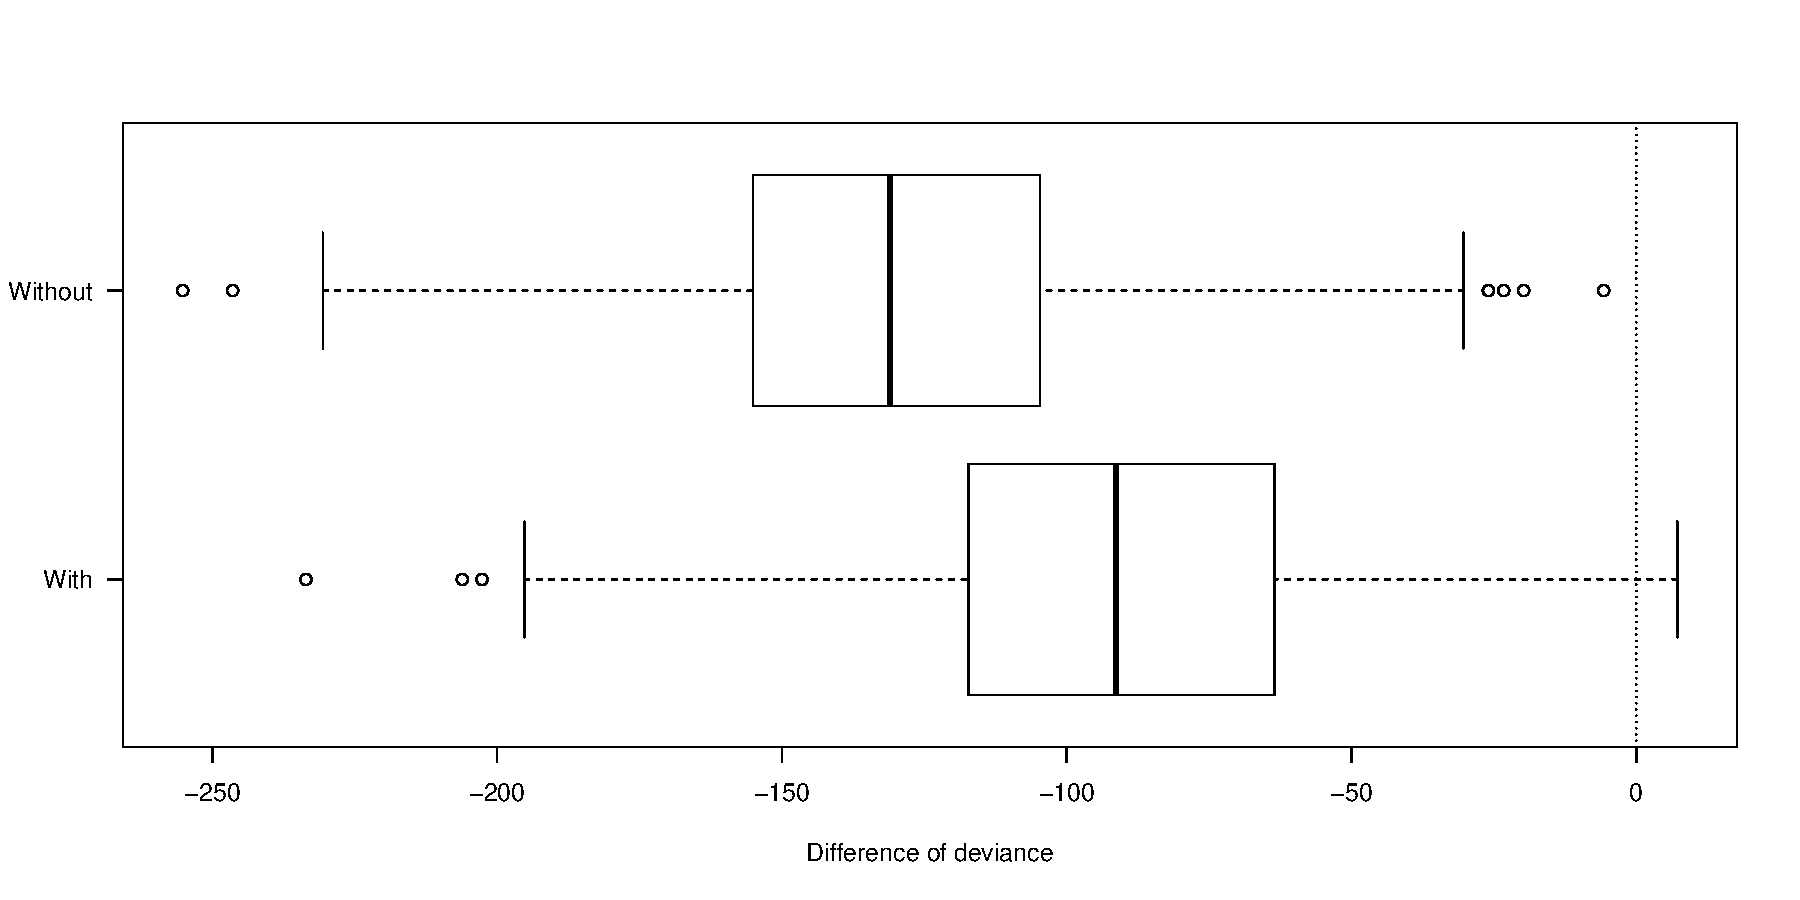
\includegraphics[scale=0.4]{deviances_simulation.pdf}
\end{figure}

\subsubsection{Variable selection}
Let us contrast the two versions of FHTBoost in terms of variable selection as well.
We report the results for the high-dimensional part in Table \ref{table:uncorrelated-y0}, and the low-dimensional part in Table \ref{table:uncorrelated-mu}.
This scenario has 35 informative gene covariates and 5 informative clinical covariates.
We are considering the sensitivity and specificity on both covariate vectors at the same time.
Since we are only selecting a covariate for either $\bbeta$ or $\bgamma$ in each iteration of the boosting algorithm, these scores will depend on each other.
Furthermore, since the changing intercept version has a rather low number of iterations, with a mean of 15.8, it is usually impossible to get anywhere near perfect on these metrics, as at most one new parameter is selected in each iteration, and we have 40 informative covariates in total from the two vectors.
Since the covariate vector is estimated on the training data, a likely explanation is that the changing intercept captures more of the variation in the training data.
In doing so, there is less variation to be explained by the covariates, and hence the boosting algorithm will start to overfit more quickly.

\begin{table}
\caption{High dimensional (genomic) part: Performance of FHTBoost in terms of variable selection, uncorrelated case}
\label{table:uncorrelated-y0}
\centering
\begin{tabular}{l|cc|cc}
\toprule
& \multicolumn{2}{c}{Updating} & \multicolumn{2}{c}{Fixed} \\
& Mean & Standard error & Mean & Standard error \\
\hline
Sensitivity & 0.190 & (0.090) & 0.452 & (0.162) \\
Specificity & 1.000 & (0.000) & 0.997 & (0.002) \\
FDR         & 0.310 & (0.176) & 0.613 & (0.144) \\
\bottomrule
\end{tabular}
\end{table}

\begin{table}
\caption{Low dimensional (clinical) part: Performance of FHTBoost in terms of variable selection, uncorrelated case}
\label{table:uncorrelated-mu}
\centering
\begin{tabular}{l|cc|cc}
\toprule
& \multicolumn{2}{c}{Updating} & \multicolumn{2}{c}{Fixed} \\
& Mean & Standard error & Mean & Standard error \\
\hline
Sensitivity & 0.741 & (0.232) & 0.958 & (0.099) \\
Specificity & 0.943 & (0.110) & 0.638 & (0.291) \\
FDR         & 0.091 & (0.144) & 0.375 & (0.192) \\
\bottomrule
\end{tabular}
\end{table}

\begin{table}
\caption{Optimal iteration number $\mstop$ results for FHTBoost, uncorrelated case}
\label{table:uncorrelated-mstop}
\centering
\begin{tabular}{l|rr}
\toprule
& Updating & Fixed \\
\hline
Mean               &  15.8  &  63.8  \\
Standard deviation &   6.4  &  26.5  \\
Minimum            &     2  &     2  \\
Maximum            &    39  &   160  \\
\bottomrule
\end{tabular}
\end{table}
Consider first the result of the version in which the intercept is changed in each step.
A very high specificity is achieved for both covariate vectors.
The specificity measures the amount of true negatives which are correctly classified as negatives, i.e., not selected.
The changing intercept version achieves a mean specificity of 1.00, and a mean false discovery rate of 0.316.
Thus there is about a one in three chance that it selects a variable which is not actually informative.
The mean sensitivity, i.e., the ratio of correctly selected informative variables, is only 0.190.
This means that a large proportion of the informative covariates are not selected.
For $\bgamma$, which is related to the clinical covariates, a much higher specificity is attained, with a mean of 0.943.
Even though the parameter effects on the drift are rather small, the informative covariates are often correctly selected.
Furthermore, the false discovery rate here is very low, with a mean of 0.091.

Now consider the results of the fixed intercept version.
For the $\bbeta$ covariate vector, a higher proportion of informative covariates are selected than the other version of FHTBoost, with a mean sensitivity of 0.452.
The mean specificity is 0.997, which is good.
Simultaneously, a larger mean false discovery rate (0.613) than the changing intercept version is not good:
An FDR of 0.613 means that more than half of all selected variables should be expected to be false positives.
At the same time, a very good sensitivity is achieved on the $\bgamma$ covariate vector, with a mean of 0.958, and a good specificity with a mean of 0.638.
The false discovery rate on $\bgamma$ is slightly above one in three, with a mean of 0.375.

\subsubsection{Summary}
Both FHTBoost versions increase the model fit when including covariates, in almost all cases.
Both also suffer from a high false discovery rate.
This issue has been raised many times before \citep{buhlmann2007, buhlmann-yu, thomas2018}.
It may especially be a problem in a setting such as ours where we have two parameters which are dependent on covariates, as it may lead to overfitting.
It also seems that the changing intercept version overfits more than the fixed intercept version, since it is allowed to change the intercept.
One remedy may be to use base learners which incorporate intercepts, as this allows also the additional intercepts to be added with the step length $\nu$.

\subsection{Scenario 2: Correlated case}
We now consider the results for the correlated simulation study.

\subsubsection{Model fit on the test set}
We observe in Figure \ref{fig:simulation-correlated-deviances-boxplot}, which is a boxplot of the deviances in this scenario, that the mean deviance is slightly better for the fixed intercept version, and with better extreme values, both minimum and maximum.
The mean deviance for the fixed intercept version is -58.8, while it is -57.8 for the changing intercept version, and both have high variability.
We should therefore not say that there is any difference in their performance with regard to model fit in this scenario.
One explanation for the equal performance in this scenario might be that since both boosting algorithm stop rather quickly (i.e. small $\mstop$) in this scenario, the intercept is allowed to change less than in scenario 1, and thus there is less overfitting.

\begin{figure}
\caption{Boxplot for difference in deviance for the two intercept variants in the correlated scenario.
The boxes are without and with changing the intercept.}
\label{fig:simulation-correlated-deviances-boxplot}
\centering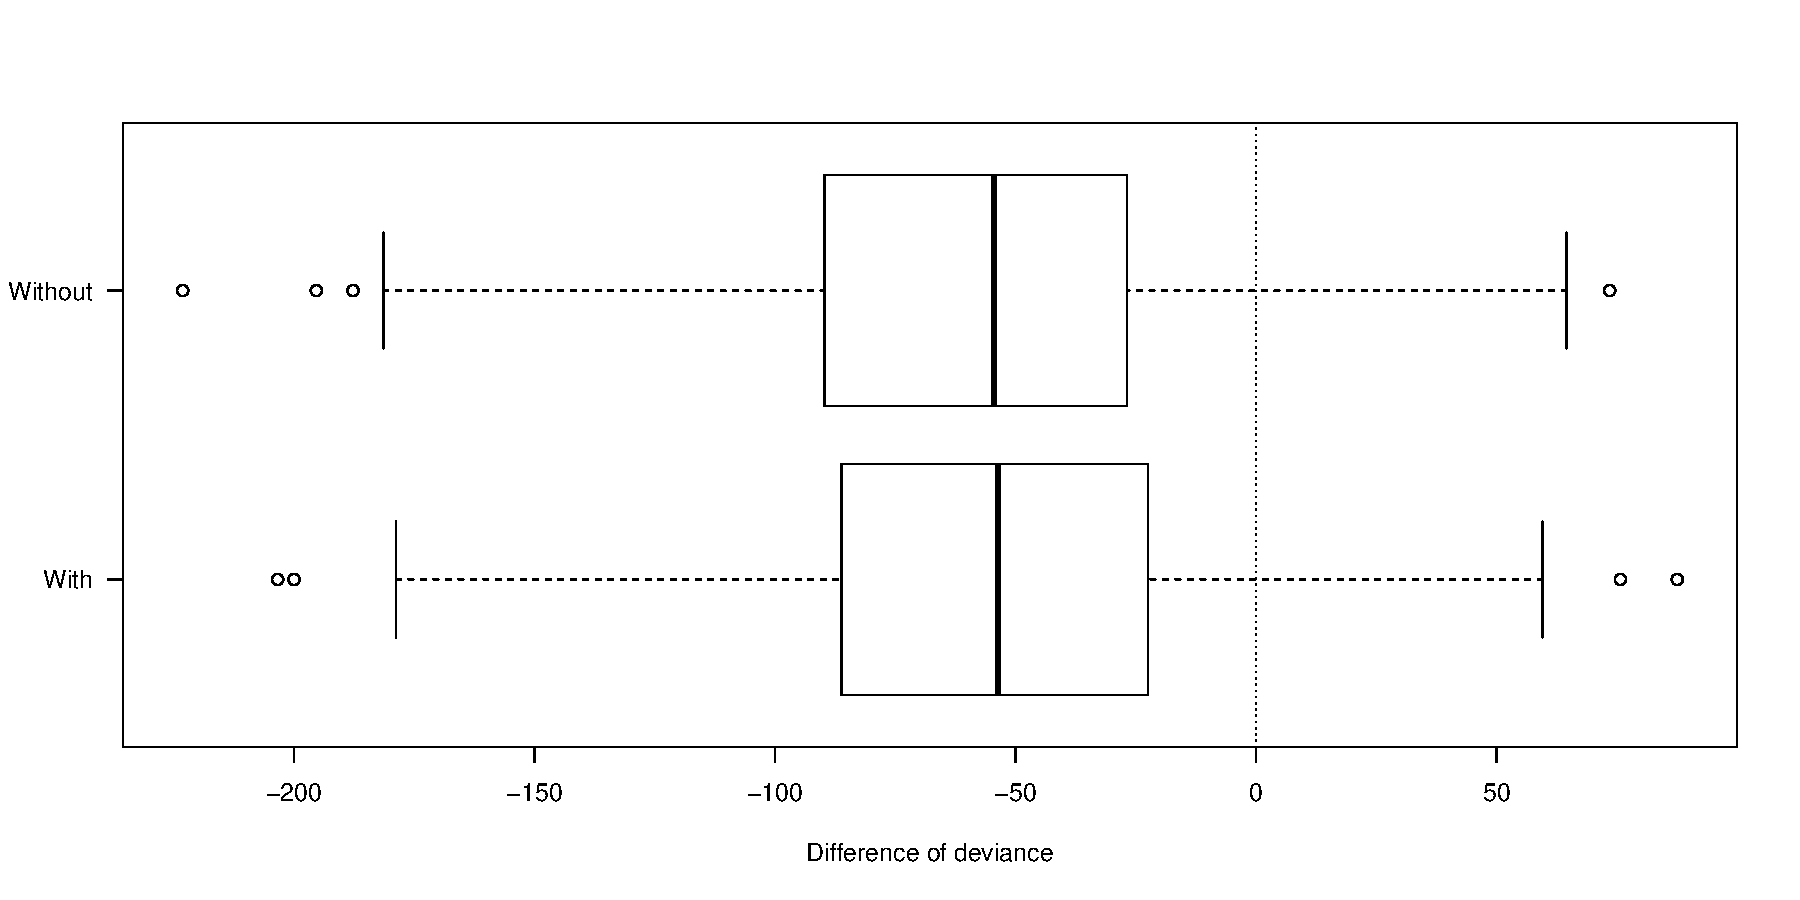
\includegraphics[scale=0.4]{deviances_simulation_correlated.pdf}
\end{figure}


\begin{table}
\caption{Difference of deviance results for FHTBoost, correlated case}
\label{table:uncorrelated-deviance}
\centering
\begin{tabular}{l|rr}
\toprule
& Updating & Fixed \\
\hline
Mean               &  -57.8  &  -58.8  \\
Standard deviation &   47.2  &   46.1  \\
Minimum            & -203.4  & -223.1  \\
Maximum            &   87.6  &   73.5  \\
\bottomrule
\end{tabular}
\end{table}


\subsubsection{Variable selection}
We now consider the variable selection metrics.
We first look at the covariate vector $\bbeta$ (see Table \ref{table:correlated-y0}), which affects the initial level $y_0$, and which is related to ``genomic'' variables.
The fixed intercept version is slightly better with regards to sensitivity, with a mean of 0.204 versus a mean of 0.157 for the changing intercept version.
So selecting informative variables,
This does come at the cost of a higher false discovery rate, with a mean as high as 0.652.
Here the changing intercept version has a mean of 0.439.
The specificity score is almost perfect in both cases.

We now consider the ``clinical'' covariates, used in $\bgamma$ and related to the drift $\mu$.
The results for it are reported in Table \ref{table:correlated-mu}.
The changing intercept version performs quite a lot worse here than the fixed intercept version, overall.
It achieves a mean sensitivity of 0.273, while the fixed intercept version achieves 0.625.
However, the changing intercept then achieves a mean of 0.831 for specificity, where the fixed intercept version attains 0.537.
For the false discovery rate, the fixed intercept has a slightly higher mean, at 0.507, whereas the changing intercept version has a mean of 0.454.

For this scenario, as well, we observe that the fixed intercept version has a higher optimal iteration number.
The mean $\mstop$ is 50 with a fixed intercept, compared to a mean of 19.5 for the changing intercept version.
Again this necessarily means that more variables are selected, and that coefficients from the changing intercept version will be more shrunken.

\begin{table}
\caption{High dimensional (genomic) part: Performance of FHTBoost in terms of variable selection, correlated case}
\label{table:correlated-y0}
\centering
\begin{tabular}{l|cc|cc}
\toprule
& \multicolumn{2}{c}{Updating} & \multicolumn{2}{c}{Fixed} \\
& Mean & Standard error & Mean & Standard error \\
\hline
Sensitivity & 0.157 & (0.084) & 0.204 & (0.081) \\
Specificity & 0.999 & (0.000) & 0.998 & (0.001) \\
FDR         & 0.439 & (0.218) & 0.652 & (0.181) \\
\bottomrule
\end{tabular}
\end{table}

\begin{table}
\caption{Low dimensional (clinical) part: Performance of FHTBoost in terms of variable selection, correlated case}
\label{table:correlated-mu}
\centering
\begin{tabular}{l|cc|cc}
\toprule
& \multicolumn{2}{c}{Updating} & \multicolumn{2}{c}{Fixed} \\
& Mean & Standard error & Mean & Standard error \\
\hline
Sensitivity & 0.273 & (0.187) & 0.625 & (0.245) \\
Specificity & 0.831 & (0.139) & 0.537 & (0.236) \\
FDR         & 0.454 & (0.250) & 0.507 & (0.130) \\
\bottomrule
\end{tabular}
\end{table}

\begin{table}
\caption{Optimal iteration number $\mstop$ results for FHTBoost, correlated case}
\label{table:correlated-mstop}
\centering
\begin{tabular}{l|rr}
\toprule
& Updating & Fixed \\
\hline
Mean               &  20.0  &  51.1  \\
Standard deviation &  12.1  &  24.4  \\
Minimum            &     2  &     2  \\
Maximum            &    65  &   148  \\
\bottomrule
\end{tabular}
\end{table}

\subsubsection{Summary}
We would expect that there would in general be higher false discovery rates in this scenario, since the data are correlated, and thus covariates which are not really informative actually often carry signal.
This was, however, not the case.
Both versions achieve practically the same deviance.
As for variable selection, while the fixed intercept version also here selects more true positive variables, it comes at a cost of selecting more false positives.

\section{Conclusion}
In general, we see that FHTBoost is able to estimate FHT models which achieve good performance, on data generated from a true FHT mechanism.
The performance achieved is especially high for the uncorrelated scenario, which is to be expected.
As we have discussed, the variable selection has trade offs.
The fixed intercept version selects more true positives, but it also selects more false positives.
It does seem to be worth it, in the end, since it achieves a better test error, i.e. a lower difference of deviance.
The results are also encouraging in the highly correlated scenario.
Since this is a much more realistic scenario, we should give more weight to the results attained in it.
If so, it is difficult to make a conclusive statement on which version is better, as the results are very similar in the highly correlated scenario.
However, to narrow down the scope of the next chapter, we will decide to only use the fixed intercept version, as we at least cannot say that the changing intercept bersion is better.